\chapter{Scientific Background}


\section{CMB Observables and the Role of Instrumental Noise}

The LiteBIRD satellite is designed to measure the anisotropies of the Cosmic Microwave Background (CMB) through the three relevant Stokes parameters: the temperature anisotropy $T$, the linear polarization components $Q$ (horizontal/vertical) and $U$ (diagonal).

LiteBIRD detectors do not measure temperature directly; instead, they measure the radiative intensity (or absorbed power) of the incoming electromagnetic radiation, integrated over finite frequency bands and for specific polarization states. From the measured intensity and intensity differences, the Stokes parameters $I, Q,$ and $U$ are reconstructed. In the context of CMB observations, the total intensity $I$ is conventionally expressed as a temperature anisotropy $T$.

Since the CMB temperature fluctuations are very small compared to the mean CMB temperature $T_{\mathrm{CMB}} \simeq 2.725\,\mathrm{K}$, the conversion from intensity to temperature is performed using the linearized Planck law. For a given frequency $\nu$, the relation between intensity fluctuations $\Delta I_\nu$ and temperature fluctuations $\Delta T$ is
\begin{equation}
\Delta I_\nu =
\left.\frac{dB_\nu(T)}{dT}\right|_{T=T_{\mathrm{CMB}}} \Delta T ,
\end{equation}
where $B_\nu(T)$ is the Planck blackbody spectrum,
\begin{equation}
B_\nu(T) = \frac{2 h \nu^3}{c^2} \frac{1}{e^{h\nu/(k_B T)} - 1}.
\end{equation}
Using this relation, the measured intensity fluctuations are converted into maps of $T, Q,$ and $U$, which are typically expressed in units of $\mu\mathrm{K}_{\mathrm{CMB}}$.

Each of the resulting sky maps $X(\hat{n}) = \{T(\hat{n}), Q(\hat{n}), U(\hat{n})\}$ can be expanded in spherical harmonics. For the temperature field, the expansion reads
\begin{equation}
T(\hat{n}) = \sum_{\ell=0}^{\infty} \sum_{m=-\ell}^{\ell} a^{T}_{\ell m} \, Y_{\ell m}(\hat{n}) .
\end{equation}

The linear polarization fields $Q(\hat{n})$ and $U(\hat{n})$ are not scalar quantities, but components of a spin-2 field on the sphere. For this reason, they are conveniently combined into the complex quantities $Q(\hat{n}) \pm iU(\hat{n})$, which can be expanded in terms of spin-weighted spherical harmonics:
\begin{equation}
Q(\hat{n}) \pm iU(\hat{n}) =
\sum_{\ell=2}^{\infty} \sum_{m=-\ell}^{\ell}
\left( a^{E}_{\ell m} \pm i a^{B}_{\ell m} \right)
\, {}_{\pm 2}Y_{\ell m}(\hat{n}) .
\end{equation}
This decomposition naturally defines the scalar E-mode and B-mode polarization components.

From the harmonic coefficients $a^{X}_{\ell m}$, the angular power spectra are defined as
\begin{equation}
C_\ell^{XY} = \frac{1}{2\ell + 1} \sum_{m=-\ell}^{\ell}
\left\langle a^{X}_{\ell m} \, a^{Y*}_{\ell m} \right\rangle ,
\end{equation}
where $X,Y \in \{T,E,B\}$. In particular, the $C_\ell^{BB}$ power spectrum quantifies the amount of B-mode polarization as a function of the multipole $\ell$, corresponding to different angular scales on the sky.

\begin{figure}[htbp]
    \centering
    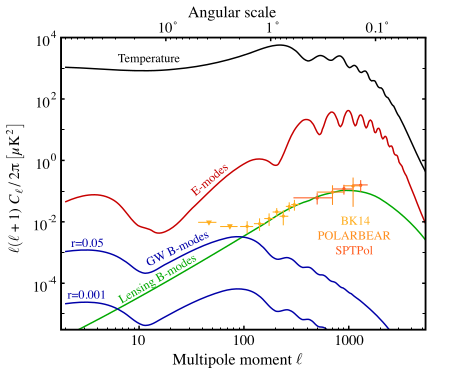
\includegraphics[width=0.68\textwidth]{2_theory_spectra.png}
    \caption{Theoretical predictions for CMB temperature, $E$-mode, and $B$-mode polarization power spectra. The plot highlights the faintness of the primordial $B$-mode signal (blue curves for different values of $r$) compared to the lensing-induced $B$-modes (green) and the dominant temperature anisotropies.}
    \label{fig:theory_spectra}
\end{figure}

The reconstruction of the CMB temperature and polarization fields does not start from direct sky maps, but from TOD streams produced by the detectors as the instrument scans the sky. Each detector sample corresponds to a measurement at a given time, pointing direction, and polarization orientation, and can be modeled as the sum of a sky signal and an instrumental noise contribution.

For a polarized detector observing the sky at time \( t \), the measured signal can be written schematically as
\begin{equation}
y_t = I_p + Q_p \cos(2\psi_t) + U_p \sin(2\psi_t) + n_t ,
\end{equation}
where \( I_p, Q_p, U_p \) are the Stokes parameters of the sky pixel \( p \), \( \psi_t \) is the detector polarization angle, and \( n_t \) denotes the instrumental noise. This relation can be compactly expressed in matrix form as
\begin{equation}
y = Ax + n,
\end{equation}
where \( y \) contains the TOD samples, \( x \) represents the pixelized sky map, \( A \) is the pointing matrix, and \( n \) is the noise vector \cite{Tegmark2001,Ashdown2007}.

In CMB experiments, each sky pixel is observed multiple times with different detector orientations, allowing the sky signal to be reconstructed from the redundant measurements. The statistical properties of the instrumental noise determine how individual samples are combined in the final map.

In realistic observations, however, instrumental noise is not purely uncorrelated. While part of the noise can be approximated as white, a significant fraction exhibits long-range temporal correlations associated with low-frequency instabilities in the detectors and readout system. If not properly modeled and mitigated, correlated noise can introduce large-scale artifacts in the reconstructed maps, posing a major challenge for polarization experiments targeting the large angular scales relevant for B-mode measurements.

The statistical properties of instrumental noise are conveniently described in the frequency domain through its power spectral density (PSD), which characterizes its temporal correlations \cite{Ashdown2007}. In particular, low-frequency noise components can couple at large angular scales in the sky through the scanning strategy, leading to excess power at low multipoles if not properly considered. For this reason, an accurate modeling of instrumental noise are essential for CMB experiments such as LiteBIRD, whose primary scientific goal is the measurement of the extremely weak B-mode polarization signal.

An important aspect of low-frequency instrumental noise is that its impact on the reconstructed maps is not easily distinguishable from cosmological signals. Because CMB observations are obtained from TOD through a scanning strategy, temporal fluctuations in the detector output are mapped onto angular fluctuations on the sky. In particular, noise components that vary slowly in time correspond to structures that are coherent over large angular scales. In harmonic space, these large-scale features project onto low multipoles $\ell$, the same regime where the primordial CMB signal carries most of its information. As a result, correlated low-frequency noise can mimic true cosmological anisotropies at low $\ell$, rather than simply adding random fluctuations. This degeneracy between instrumental noise and sky signal makes the control and mitigation of low-frequency noise a critical requirement for experiments such as LiteBIRD, which aim to measure extremely weak B-mode polarization on large angular scales.




\section{White Noise and $1/f$ Noise}

The output of any detector inevitably contains statistical noise, which limits the sensitivity of the measurements. Instrumental noise can be classified into two main components: uncorrelated (white) noise and correlated ($1/f$) noise. Each type of noise affects the measurement in different ways and must be properly characterized to understand its impact on the reconstructed sky maps.

\begin{figure}[htbp]
     \centering
     \begin{subfigure}[b]{0.38\textwidth}
         \centering
         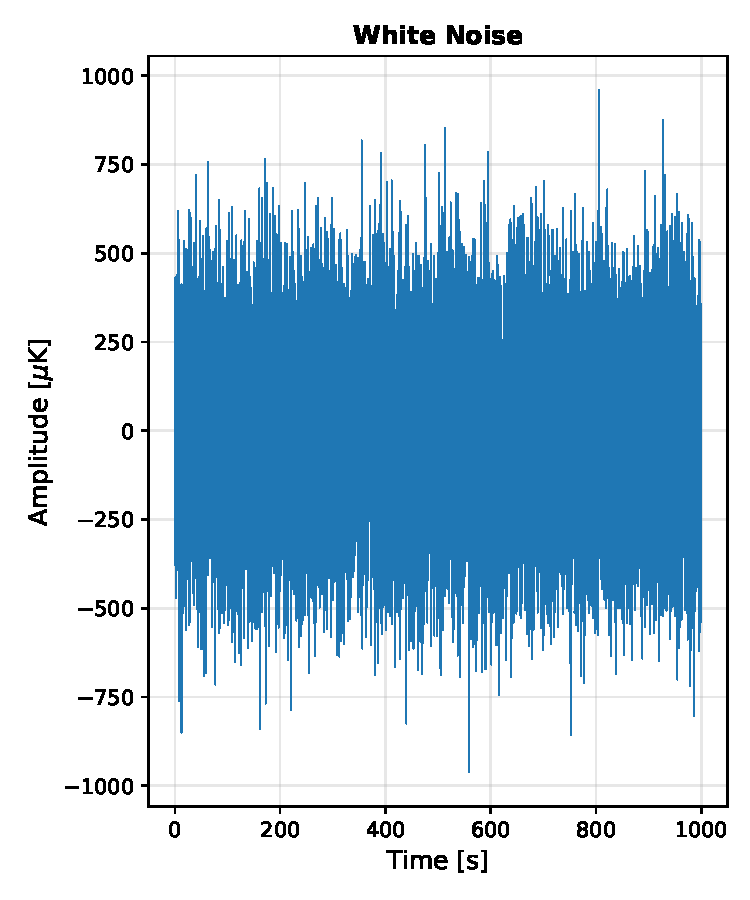
\includegraphics[width=\textwidth]{2_white.pdf}
         \label{fig:white_noise}
     \end{subfigure}
     \hspace{3mm} 
     \begin{subfigure}[b]{0.38\textwidth}
         \centering
         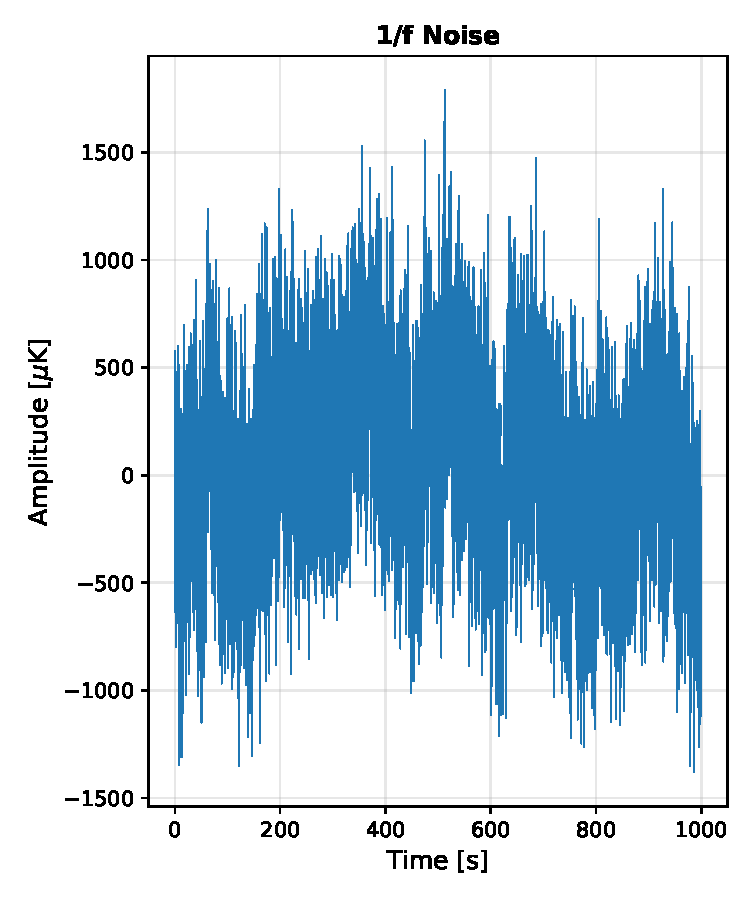
\includegraphics[width=\textwidth]{2_1overf.pdf}
         \label{fig:one_over_f}
     \end{subfigure}
     \caption{Comparison of noise realizations in the time domain. Left: White Gaussian noise, characterized by independent samples and a flat spectrum. Right: Correlated $1/f$ noise, showing slow low-frequency drifts that can be misinterpreted as large-scale cosmological signals.}
     \label{fig:noise_comparison}
\end{figure}

\subsection{White Noise}
White noise is a stochastic process with a flat power spectral density (PSD), meaning that all temporal frequencies contribute equally to the signal. In discrete time, white noise can be represented as a sequence of statistically independent random variables with zero mean and finite variance. If the samples are normally distributed, the noise is referred to as additive white Gaussian noise.

Mathematically, white noise satisfies
\begin{equation}
\langle n(t) \rangle = 0, \qquad
\langle n(t)n(t') \rangle = \sigma^2 \delta(t-t'),
\end{equation}
where $\sigma^2$ is the white noise level. Its PSD is therefore constant over frequency:
\begin{equation}
P(f) = \sigma^2.
\end{equation}

Two key properties of white noise are:
\begin{enumerate}
    \item Flat spectrum: all frequencies contribute equally to the signal power.
    \item No temporal correlation: samples at different times are statistically independent.
\end{enumerate}

It is important to note that Gaussianity and whiteness are distinct concepts. Gaussianity refers to the probability distribution of the signal amplitude, while whiteness refers to the distribution of power across frequencies. A signal can be Gaussian but not white, or white but not Gaussian.


\subsection{1/f Noise}
$1/f$ noise, also known as pink noise, is a low-frequency correlated component, commonly observed in microwave detectors and radio receivers. Unlike white noise, $1/f$ noise exhibits long-term correlations, causing slow drifts in the detector output. Its PSD follows an approximate power-law behavior:
\begin{equation}
P(f) = \sigma^2 \left(\frac{f_{knee}}{f}\right)^\alpha,
\end{equation}
where $f_{knee}$ is the knee frequency, $\alpha$ is the spectral index (typically between 1 and 2), and $\sigma^2$ is the white noise level. Below $f_{knee}$, the $1/f$ component dominates, while above $f_{knee}$ the noise becomes effectively white. This behavior introduces excess power at low frequencies, which projects onto large angular scales in sky maps and can significantly affect B-mode polarization measurements.

In practical terms, $1/f$ noise arises from slow instabilities in the detector or the readout electronics, often related to thermal or electronic fluctuations. Its presence motivates the use of stable cryogenic systems and careful calibration to minimize drifts and gain fluctuations.

In summary, white noise contributes equally at all temporal frequencies and is uncorrelated over time, while $1/f$ noise dominates at low frequencies and exhibits long-term correlations. Understanding the statistical differences between these two noise components is essential for designing realistic simulations of time-ordered data and for predicting their impact on the reconstructed sky maps.





\section{Power Spectral Density}

The power spectral density (PSD) describes how the power of a signal is distributed across frequencies. In CMB studies, it is a fundamental tool to characterize instrumental noise. The PSD provides insight into the frequency-dependent behavior of the noise.


\subsection{PSD Estimation with the FFT}
A simple approach to estimate the PSD is based on the discrete Fourier transform (DFT) of a sampled signal \cite{press2007numerical}. For a time series sampled at $N$ points $c_0, \dots, c_{N-1}$, the DFT is

\begin{equation}
C_k = \sum_{j=0}^{N-1} c_j \, e^{2\pi i jk / N}, \quad k = 0, \dots, N-1.
\end{equation}

The periodogram estimates the PSD as the squared modulus of the DFT:

\begin{equation}
P(f_k) = \frac{1}{N^2} |C_k|^2, \quad k = 0, \dots, \frac{N}{2}.
\end{equation}

This gives the power associated with positive frequencies $f_k = k / (N \Delta)$, where $\Delta$ is the sampling interval. While straightforward, the periodogram suffers from spectral leakage, where power from one frequency spreads into neighboring bins. Leakage arises because a finite-length segment of data is effectively multiplied by a square window in time, whose Fourier transform contains high-frequency components.

To reduce leakage, each data segment can be multiplied by a window function $w_j$ that smoothly rises and falls at the segment edges. The resulting windowed periodogram is

\begin{equation}
D_k = \sum_{j=0}^{N-1} c_j w_j \, e^{2\pi i jk / N}, \quad
P(f_k) = \frac{1}{\sum_j w_j^2} |D_k|^2.
\end{equation}

Common windows include Hann, Hamming, and Bartlett. Windowing suppresses leakage but slightly increases the variance of the PSD estimate, since data near the edges are down-weighted \cite{press2007numerical}.


\subsection{Welch's Method}

Welch's method improves the PSD estimate by splitting the signal into overlapping segments, applying a window to each, computing their periodograms, and averaging them. This approach reduces variance compared to the simple periodogram and maintains low leakage. Typical overlap is 50\% of the segment length.

The main steps of Welch's method are:

\begin{enumerate}
    \item Segmenting the signal: the signal is divided into partially overlapping segments to increase the number of independent estimates.
    \item Windowing: each segment is multiplied by a window function (e.g., Hann or Hamming) to reduce edge effects. The window suppresses spectral leakage, i.e., the spreading of power from a frequency to neighboring frequencies.
    \item Fourier Transform: the FFT of each windowed segment is computed.
    \item Power computation: the local periodogram of each segment is obtained as the squared modulus of the FFT.
    \item Averaging: the periodograms of all segments are averaged to obtain the final PSD.
    \begin{itemize}
        \item Averaging reduces the variance of the estimate, smoothing fluctuations around the mean.
        \item As a side effect, the frequency resolution is reduced.
    \end{itemize}
\end{enumerate}

In Python, \texttt{scipy.signal.welch()} performs these steps efficiently, taking a time series and returning its PSD.

When a segment of the signal is treated as zero outside its boundaries, the FFT of the segment corresponds to the Fourier transform of the signal multiplied by a characteristic function $\chi$, which results in a frequency spread around the central frequency $\nu_0$ instead of a Dirac delta. By multiplying the segment by a window function, the resulting PSD is effectively the convolution of the signal's Fourier transform with the Fourier transform of the window. This softens the spectral distribution and further reduces leakage, providing a more accurate estimate of the PSD.

The PSD obtained in this way quantifies the power in each frequency band, which is essential for analyzing instrumental noise in CMB simulations.





\section{HEALPix Sky Pixelization}

Many experiments in observational cosmology, and in particular studies of the Cosmic Microwave Background (CMB), produce data that naturally live on the surface of a sphere. In order to analyze such data numerically, it is necessary to introduce a discretized representation of the sky, i.e., a pixelization of the sphere.

A pixelization scheme widely adopted in CMB data analysis is HEALPix, short for \textit{Hierarchical Equal Area isoLatitude Pixelization} of the sphere, introduced by Górski et al.~\cite{Gorski2005}. HEALPix was specifically designed to meet the requirements of full-sky cosmological observations and has become a standard tool in modern CMB experiments.

The HEALPix scheme is characterized by three key features:

\begin{itemize}
    \item Equal-area pixels, ensuring that each pixel covers the same solid angle on the sky. This property prevents spatial variations in noise level due solely to the pixelization and guarantees that white instrumental noise remains white after projection into map space.
    \item Hierarchical structure, which allows the sky resolution to be increased by recursively subdividing pixels. This is particularly advantageous for handling large data sets and enables efficient memory management and multiresolution analyses.
    \item Iso-latitude pixel centers, meaning that pixels are arranged in rings of constant latitude. This feature is crucial for enabling fast spherical harmonic transforms, which are central to CMB data analysis.
\end{itemize}

\begin{figure}[htbp]
    \centering
    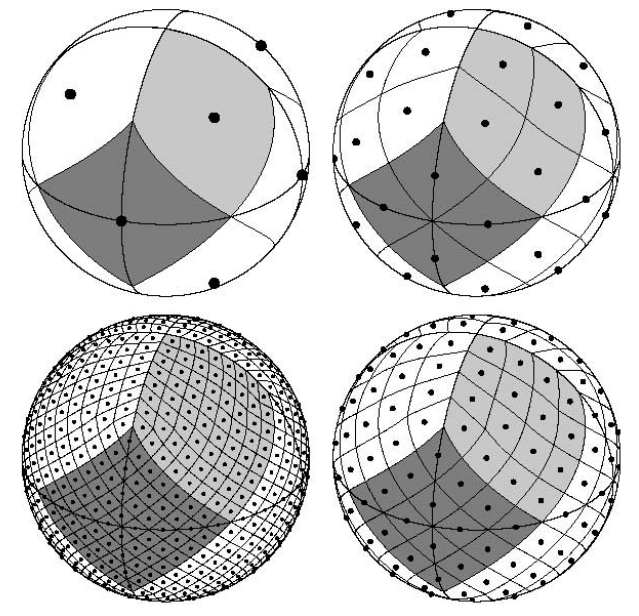
\includegraphics[width=0.45\textwidth]{2_healpix.png}
    \caption[Orthographic view of the HEALPix partition]{Orthographic view of the HEALPix partition of the sphere. The sequence illustrates the hierarchical subdivision of the 12 base-resolution pixels as the resolution parameter $N_{side}$ increases ($N_{side} = 1, 2, 4, 8$), maintaining equal-area properties for all pixels. Image taken from \cite{Gorski2005}.}
    \label{fig:healpix_hierarchy}
\end{figure}

At the lowest resolution, HEALPix divides the sphere into 12 base pixels of equal area. This base tessellation is constructed by partitioning the sphere into 3 regions in latitude: a northern polar cap, an equatorial region, and a southern polar cap. Each of these regions is further divided into 4 pixels in longitude, resulting in a total of $3 \times 4 = 12$ base pixels.

The resolution of a HEALPix map is controlled by a single integer parameter, \texttt{Nside}, which specifies how many times each side of a base pixel is subdivided. Increasing \texttt{Nside} increases the angular resolution of the map while preserving the equal-area and hierarchical properties of the pixelization.

The total number of pixels in a HEALPix map is given by:
\begin{equation}
N_{\text{pix}} = 12\,N_{\text{side}}^{2}.
\end{equation}

Each pixel covers the same solid angle:
\begin{equation}
\Omega_{\text{pix}} = \frac{4\pi}{N_{\text{pix}}} = \frac{\pi}{3\,N_{\text{side}}^{2}}.
\end{equation}

Practical applications require choosing an appropriate value of \texttt{Nside}. Increasing the resolution improves angular fidelity but also leads to: higher memory usage, longer computation times, larger time-ordered and map-level data products.
